%\RequirePackage[l2tabu, orthodox]{nag}
\documentclass[a4paper,12pt]{scrreprt}
\usepackage[utf8]{inputenc}   % input encoding
\usepackage[T1]{fontenc}      % font encoding
\usepackage[english]{babel}		% English language 
\usepackage[backend=bibtex,style=authoryear,bibstyle=nature,natbib=true]{biblatex}
\usepackage{lmodern}					% font looks better on screen
\usepackage{microtype}				% improve kerning
\usepackage{color}						% enable color
% if using natbib
%\usepackage{natbib}           % bibliography for scientists
% if using biblatex
\usepackage{csquotes}         % dunno what this does
%--------------------------------------------------
% more features
\usepackage{graphicx}					% fancy graphics
%\usepackage{enumerate}				% customize numbered lists
\usepackage{amsmath}					% all the fancy math stuff
\usepackage{listings}         % code listings
%\usepackage{tabularx}         % extended tables
%\usepackage{tikz}             % draw stuff with tikz
\usepackage{url}							% URL handling
\usepackage{xspace}						% to space or not to space
\usepackage{hyperref} 				% should be loaded last
%--------------------------------------------------

% setup biblatex
\bibliography{bib/diploma}
\ExecuteBibliographyOptions{
	firstinits=true,
	backref=true,
	isbn=false,
	url=false,
	maxcitenames=2,
	maxbibnames=999,
}
\renewcommand{\bibfont}{\normalfont\footnotesize}

% setup natbib citation format
%\bibpunct{(}{)}{,}{a}{,}{,}

% setup the listings package
\lstset{%
	language=perl,
	basicstyle=,                       % size of the fonts that are used for the code
	numbers=left,                      % where to put the line numbers
	numberstyle=\tiny,                 % size of the fonts that are used for the line numbers
	%stepnumber=2,                      % step between two line numbers. 
	numbersep=5pt,                     % how far the line numbers are from the code
	backgroundcolor=\color{lightgrey}, % choose the background color. Requires \usepackage{color}
	showspaces=false,                  % show spaces adding particular underscores
	showstringspaces=false,            % underline spaces within strings
	showtabs=false,                    % show tabs 
	frame=none,                        % none|leftline|topline|bottomline|lines|single, shadowbox 
	%frameround=tttt,                   % rounded corners; t=round, f=corner
	tabsize=2,                         % sets default tabsize to 2 spaces
	captionpos=t,                      % caption position (t|b)
	breaklines=true,                   % automatic line breaking
	breakatwhitespace=false,           % automatic breaks should not happen at whitespace
	%escapeinside={\%}{)}               % if you want to add a comment within your code
}

% setup hyperlinks, bookmarks and pdf metadata
\hypersetup{%
	bookmarks=true,
	pdfborder={0 0 0},
	pdftitle={Fast and efficient mapping of transcript sequences to ortholog groups},
	pdfauthor={Malte Petersen},
	pdfcreator={pdflatex},
	pdfsubject={orthology prediction},
	pdfkeywords={orthology} {prediction} {est} {transcriptome} {hmm} {phylogenetics} {thesis} {1kite}
}
% alleviate compression so pdftk won't complain
\pdfobjcompresslevel=1

% new colors and commands
\definecolor{lightgrey}{rgb}{0.9,0.9,0.9}
\newcommand{\file}[1]{{\lstinline{#1}}}
\newcommand{\code}[1]{{\texttt{#1}}}
\newcommand{\hamstr}{HaMStR\xspace}
\newcommand{\pname}{Orthograph\xspace}
\newcommand{\species}[1]{\textit{#1}}
\newcommand{\todo}[1]{\textbf{\color{red}[#1]}}

% doublespace
\linespread{1.3}

\title{Fast and efficient mapping of transcript sequences to ortholog groups}
\author{Malte Petersen}

\begin{document}
\maketitle
\pagestyle{headings}
\tableofcontents

\chapter*{Paper notes}
	Strategies for orthology prediction:

Tree-based and graph-based approaches: advantages and pitfalls

\begin{description}
	\item[\cite{mirkin1995}] Tree-based approach to orthology prediction
	\item[\cite{yuan1998}] Tree-based approach to orthology prediction
	\item[\cite{kuzniar2008}] Review of approaches
\end{description}

Graph-based approaches:

Triangulation

\begin{itemize}
	\item OrthoDB 
	\item COG (KOG, EGO, etc)
\end{itemize}

Reciprocal best hit (RBH) 

\begin{itemize}
	\item InParanoid (BLAST based)
\end{itemize}

Markov clustering:

\begin{itemize}
	\item OrthoMCL
\end{itemize}



\thispagestyle{empty}
\null
\vfill
%--------------------------------------------------
% \begin{quote}
% 	\emph{Mutation:} it is the key to our evolution. It has enabled us to evolve
% 	from a single-celled organism into the dominant species on the planet. This
% 	process is slow, and normally taking thousands and thousands of years. But
% 	every few hundred millennia, evolution leaps forward.\\
% 	\null\hfill--- \citet{singer2000}
% \end{quote}
%-------------------------------------------------- 
\begin{quote}
The Haggunenons of Vicissitus Three have the most impatient chromosomes of any
life form in the Galaxy. Whereas most races are content to evolve slowly and
carefully over thousands of generations, discarding a prehensile toe here,
nervously hazarding another nostril there, the Haggunenons would do for Charles
Darwin what a squadron of Arcturan stunt apples would have done for Sir Isaac
Newton. Their genetic structure, based on the quadruple sterated octohelix, is
so chronically unstable, that far from passing their basic shape onto their
children, they quite frequently evolve several times over lunch. But they do
this with such reckless abandon that if, sitting at table, they are unable to
reach a coffee spoon, they are liable without a moment's consideration to mutate
into something with far longer arms \dots but which is probably quite incapable
of drinking coffee.\\
\null\hfill--- The Hitchhiker's Guide to the Galaxy \citep{adams1979}
\end{quote}


\chapter{Introduction}
	Since the advent of molecular sequencing techniques and the reconstruction of
phylogenies based on nucleic or amino acid sequences, homology is still a
required, but no longer a sufficient criterion for comparing characters.
So-called orthologs allow retracing speciation events in a phylogenetic context.
Common orthology prediction techniques that are applied to genomes or proteomes,
however, cannot be applied to transcriptomic sequence data because of its
inherent incompleteness. In the present thesis, I establish a software pipeline
for orthology prediction in transcriptome data.



	\section{Orthology}
		When reconstructing species lineages, so called homologous characters are used
to reconstruct ancestral trees. The term homolog was introduced in 1848
(\cite{owen1848}) and was used to describe ``the same organ in different animals
under different every variety of form and function''. Similarly, analogs were
defined as ``part or organ in one animal which has the same function as another
part or organ in a different animal''. At that time, Owen had no notion of the
concept of evolution, and in the famous \emph{Origin of Species}
(\cite{darwin1859}), the term homology is never used, but in a review
(\cite{owen1860}), he refers to homology as evidence of evolution.

A morphological character is the phenotypic reflection of a molecular character.
Molecular characters, such as genes, are homologous if they share a common
origin (\cite{koonin2005}). However, this is not sufficient to infer reliable
phylogenies based on molecular data. Genes can be subject to a number of events
in the course of their evolutionary history, such as speciation, gene
duplication, gene loss, horizontal gene transfer and fusion, fission and other
rearrangements of genes. These different types of relatedness between molecular
sequences have made new definitions necessary (see figure \ref{fig:orthology}).

\begin{figure}[h]
	\centering
	\def\svgwidth{0.8\textwidth}
	\input{img/orthology-paralogy.pdf_tex}
	\caption[Orthology, paralogy, and xenology]{Subtypes of homology. The red
		arrow denotes horizontal gene transfer; AB1 is \emph{xenologous} to all
		other genes. B1 and C1 are \emph{orthologs}. Both C2 and C3 are
		\emph{inparalogs} to each other but \emph{co-orthologs} to B2, as are B1 and
		C1 compared to A1. B1 and B2 are outparalogs. Graphic adapted from
		\citet{fitch2000}.
	}
	\label{fig:orthology}
\end{figure}


Homologous genes that are related by a speciation event are called
\emph{orthologs} (\cite{fitch1970}). They reflect species phylogeny directly and
are most commonly used to infer species lineages. \emph{Paralogous} genes are
also homologous, but they are related by a gene duplication event and are not
involved in horizontal radiation. Further distinction must be made among
paralogous genes (\cite{sonnhammer2002}): paralogous genes that are related by a
lineage-specific duplication are called \emph{outparalogs} if the duplication
occurred prior to a given speciation event, while genes that result from a
lineage-specific duplication subsequent to a given speciation event are called
\emph{inparalogs}.  These distinctions are important when looking at internal
branches of a phylogenetic tree.

The fourth subtype of homology that is called \emph{xenology}. It is defined as
the condition where the history of the gene involves horizontal, or
interspecies, gene transfer (\cite{gray1983}). This is the only form of homology
in which the gene lineage cannot be traced back to a parent, but instead from
one organism to another.

In molecular phylogenetics, ortholog characters are used to reconstruct species
lineages, because these sequences are the only homologous sequences whose
phylogeny reflects exactly the true phylogeny of the species from which the
sequences were obtained. Orthologs are also used to study mechanisms of gene and
genome evolution (\cite{dessimoz2012}). Orthologs tend to be more functionally
similar than paralogs (\cite{altenhoff2012}); this emphasizes the so-called
\emph{ortholog conjecture} (\cite{tatusov1997}) and is the reason why the
analysis of protein families often requires orthology among the investigated
genes.




Since molecular genetics entered the field of phylogenetics during the 1960s,


	\section{How can orthology be assessed?}
		With next-generation, high-throughput technologies providing vast amounts of
sequence data, 

To make use of the information contained in the ortholog property, it is
important to classify conserved genes according to their homologous
relationships. It is worth mentioning here that homology is a concept of
quality, not quantity (\cite{reeck1987}) and thus indivisible. Two sequences can
be \emph{similar} by a percentage (e.g., amino acid positional identity), but
they are either homologous or they are not. The same follows for orthologs,
paralogs, and xenologs. This distinction is important because homology implies a
genealogical relationship, whereas similarity does not. Similarity can also be
the result of other evolutionary processes, such as convergence, which results
in \emph{analogy}. All variants of similarity can be grouped under the term
\emph{homoplasy}, which encompasses similarity (\emph{homos} (``equal''),
\emph{plasis} (``shaping'')) excluding homology and its subforms. In the present
thesis, the definition of homoplasy is used as it appears in \cite{page1998}.

A simple alignment or scoring (i.e., similarity) alone cannot separate
homologous from merely similar sequences (\cite{eisen1998}). To distinguish
homology from homoplasy, further logic is necessary: 

See figure \ref{fig:hamstr}.

	\section{Transcriptomes and additional challenges}
		Going a step back and asking why genomes are studied, many times the answer is
that one wants to understand the function of genes and proteins. The genome is
made up of long strands of deoxyribonucleic acid (DNA). It contains the
necessary instructions to create and maintain cells.  Proteins are produced
according to information on the DNA in a two-step process: during
\emph{transcription}, messenger ribonucleic acid (mRNA) is synthetisized. In the
second step, \emph{translation}, the mRNA is used by specialized organelles,
namely ribosomes, to synthetisize proteins from amino acids. In eukaryotes, this
process includes \emph{splicing}, during which non-coding regions, so-called
\emph{introns} are removed from the mRNA. In bacteria and archaea, the mRNA
requires typically no further processing before translation. The resulting
molecule contains only \emph{exons}, coding regions of the genome that are
relevant for translation. The ratio of exons to introns varies across organisms;
e.g., the human genome consists of only 1.1\% to 1.4\% exons and 24.4\% to
37.8\% introns, the remainder is intergenic DNA \citep{venter2001}. That means
that in eukaryotes, the majority of the genome does not code for proteins, and
the functional analysis of the genes in an eukaryote genome requires screening
the nucleotide sequence data for those non-coding regions.

The study of \emph{transcriptomes} circumvents these problems. A transcriptome
is the collection of all transcripts in a tissue sample at the time of RNA
preservation.  Transcriptomes are frequently used in phylogenetics and
phylogenomics to reconstruct species trees based on hundreds of
genes\footnote{The 1KITE project (1K Insect Transcriptome Evolution,
\url{http://1kite.org}) aims to sequence the transcriptomes of 1,000 insect
species and infer a robust backbone tree of insects. Preliminary analyses were
performed on a supermatrix of 1,478 genes.}.  The combination of low-cost
next-generation sequencing and the intron-free nature of transcriptomes allow
access to a high proportion of protein coding genes per sequenced mega-base pair
at a fraction of the cost for sequencing the corresponding genome.

Next-generation transcriptome sequencing technologies achieve their high
throughput by massively parallelizing the sequencing process. They cannot
sequence whole genomes in a single run, but produce a large number of so-called
\emph{reads}, short nucleotide sequences (20 to 1,000 bp in length, depending on
the technology used). These fragments must be \emph{assembled} to form so-called
\emph{contigs}, contiguous sequences of nucleotides that most closely resembles
the nucleotide sequence present in the sequenced specimen. The assembly process
is a computationally complex problem that has not yet been solved to
perfection. Reviews of different strategies have been written by, e.g.,
\citet{zhang2011}. The assembled data may be redundant due to, e.g.,
alternative splicing products \citep{black2003} or multiple, non-overlapping
sequencing of C-terminus and N-terminus (the two ends of a DNA strand or gene).
Most assembly software cannot detect these issues reliably
\citep{haiminen2011}. 

In addition to the processes explained above, next-generation transcriptome
sequencing and assembly output sequence data are not only fragmented and
possibly redundant (overlapping), but most importantly they are
\emph{incomplete} because not all genes may have been expressed at the time of
preservation. Due to this inherent incompleteness of transcriptomes, orthology
prediction approaches that are used on fully sequenced and annotated genomes
cannot be used.

\begin{figure}[t]
	\centering
	\includegraphics[width=0.4\textwidth]{img/triangulation-bbh.pdf}
	\caption[Bidirectional best hit (BBH) triangulation]{
		BBH triangulation. To identify genes as orthologous in the presence of
		potential gene loss or incomplete data, they must be BBH in three species.
		In this example, the red gene fulfills this criterion. The blue gene cannot
		be unambiguously identified as orthologous, as it is not present in the frog
		and paralogy is possible (compare to \autoref{fig:graph-based-strat}).
		Graphic modified from \citet{altenhoff2012}.
	}
	\label{fig:triangulation-bbh}
\end{figure}


When performing a bidirectional search on a fully sequenced and annotated
complete genome as described above, it can happen that two genes that are
identified as BBH are paralogs because the corresponding orthologs have been
lost in both investigated species. This situation is called \emph{differential
gene loss} and best solved using a tree-based approach. In the face of the
aforementioned difficulties of a tree-based strategy, some graph-based
algorithms implement \emph{triangulation} (\autoref{fig:triangulation-bbh}): to
identify two genes as orthologous, they must be BBH not only in two, but in
three species. The third gene functions as possible ``witness of non-orthology''
\citep{dessimoz2006}. A triangulation strategy can also be applied to orthology
prediction in transcriptomic data, the incompleteness of which may be seen as a
similar situation as potential gene loss in fully sequenced and annotated
genomes. This approach has been implemented in \hamstr \citep{ebersberger2009},
which I will describe in the following section.

	\section{\hamstr}
		\hamstr implements a graph-based approach using profile hidden Markov models
(HMMs, explained in \autoref{sec:hmms}). It is aimed specifically at
searching for orthologs in \emph{expressed sequence tag} (EST)
data\footnote{National Center for Biotechnology Information: EST fact sheet
(\url{http://www.ncbi.nlm.nih.gov/About/primer/est.html}, revised: March 29,
2004)}, which are sequenced using complementary DNA (cDNA) libraries in a
process called \emph{shotgun sequencing}. The cDNA is cloned from mRNA and
therefore contains no introns, and, like a transcriptome, EST data is
incomplete, i.e., it contains only nucleotide sequences of the genes that were
expressed at the time of RNA preservation. Due to the way it is sequenced and
assembled, EST data can be redundant and fragmented as well, which is why
methods for orthology prediction in genomic data cannot be applied, and
approaches like described above have to be used.

\hamstr cannot be used to perform \emph{de novo} orthology assessment. Instead,
it relies on pre-computed ortholog goups that data from the query EST library is
clustered to. These so-called \emph{core orthologs} are compiled from existing
databases such as OrthoDB and must be of species for which a complete genome is
available. From each \emph{ortholog group} (OG, a set of genes that are known to
be one-to-one orthologous), a HMM is generated: each HMM is a probabilistic
representation of the amino acid sequence of a gene. 

\hamstr uses a three-step triangulation strategy as depicted in
\autoref{fig:hamstr-triangulation}: the EST sequence space is searched with the
HMMs for matches (\autoref{fig:hamstr-triangulation}a). To verify orthology in
the HMM hits, each hit sequence is compared via BLASTP \citep{altschul1997} to a
so-called reference taxon (\autoref{fig:hamstr-triangulation}b). Note that the
proteome, itself being complete, contains the amino acid sequences that are
known to be orthologous. If the BLAST search hits a sequence that was used to
generate the HMM (\autoref{fig:hamstr-triangulation}c), then orthology is
assumed and the EST in question is added to the ortholog cluster. Otherwise, it
is discarded.

\begin{figure}[t]
	\centering
	\def\svgwidth{0.8\textwidth}
	\input{img/triangulation.pdf_tex}
	\caption[Triangulation]{Triangulation:
		\textbf{a)} The transcript sequence space is searched using a hidden Markov
			model (HMM), which is a statistical representation of the reference
			sequences that were used to build it.
		\textbf{b)} A reference proteome is searched using the match sequence from the
			HMM search (reciprocal search).
		\textbf{c)} If the reciprocal search match sequence is one that was used to
			build the HMM, then orthology is assumed.
	}
	\label{fig:hamstr-triangulation}
\end{figure}




% enable this if you need it, it makes compilation a bit slower
%\usetikzlibrary{shapes,arrows}
\tikzstyle{rect} = [
	rectangle,
	draw,
	fill = green!15,
	text width = 9 em,
	text centered,
	minimum height = 3 em,
]
\tikzstyle{block} = [
	rectangle,
	draw,
	fill = blue!20,
	text width = 13em,
	text centered,
	rounded corners,
	minimum height = 3em,
]
\tikzstyle{decision} = [
	diamond,
	draw, 
	fill = blue!20, 
	text width = 4.5em,
	text centered,
	node distance = 14em,
	inner sep = 0pt
]
\tikzstyle{line} = [draw, -latex]
\tikzstyle{cloud} = [
	draw,
	ellipse,
	fill = red!20,
	text width = 7.5em,
	text badly centered,
	node distance = 3cm,
	minimum height = 2em
]

\hyphenation{ref-e-ren-ce tran-scrip-to-me or-tho-lo-gous}
\begin{tikzpicture}[node distance = 2cm, auto]
	% nodes
	\node[rect] (transcriptome) {Transcriptome library};
	\node[block, below of = transcriptome] (hmmsearch) {Search transcriptome library using next HMM};
	\node[rect, left of = hmmsearch, node distance = 14em] (orthologs) {pHMMs of orthologous sequences};
	\node[block, above of = orthologs] (orthodb) {Orthologous sequences of reference taxa from OrthoDB};
	\node[block, below of = hmmsearch, node distance = 4em] (hmmhits) {BLAST result(s) against next reference taxon};
	\node[decision, below of = hmmhits, node distance = 7em] (blast) {BLAST hit in HMM?};
	\node[rect, right of = hmmhits, node distance = 14em] (proteomes) {Proteomes of the reference taxa};
	\node[cloud, below of = blast, node distance=7em] (orthologous) {Orthologous, save \& process};
	\node[decision, below of = orthologous, node distance = 6em] (hmmsleft) {HMMs left?};
	\node[decision, left of = blast, node distance = 16em] (reftaxaleft) {Reference taxa left?};
	\node[cloud, below of = reftaxaleft, node distance = 7em] (notorthologous) {Not orthologous, discard};
	\node[draw, below of = hmmsleft, node distance = 6em] (end) {End};

	% lines
	\path[line](transcriptome) -- (hmmsearch);
	\path[line](orthodb) -- (orthologs);
	\path[line](orthologs) -- (hmmsearch);
	\path[line](hmmsearch) -- (hmmhits);
	\path[line](proteomes) -- (hmmhits);
	\path[line](hmmhits) -- (blast);
	\path[line](blast) -- node[near start]{no} (reftaxaleft);
	\path[line](blast) -- node[near start]{yes} (orthologous);
	\path[line](orthologous) -- (hmmsleft);
	\path[line](hmmsleft) -| node[near start]{yes} ([xshift = 18.0em]hmmsleft.east) |- (hmmsearch);
	\path[line](reftaxaleft) |- node[near start]{yes} (hmmhits);
	\path[line](reftaxaleft) -- node[near start]{no} (notorthologous);
	\path[line](notorthologous) |- (hmmsleft);
	\path[line](hmmsleft) -- node[near start] {no} (end);
\end{tikzpicture}


\todo{more elaboration here}

		\subsection{Hidden Markov models}
			\label{sec:hmms}
Proteins, RNAs and other biological molecular sequences can usually be
classified into families of related sequences and structures
(\cite{henikoff1997}). Since a similarity measure bears no genealogical meaning,
as explained in \autoref{sec:orthology-howto}, more appropriate approaches must
be tried.

Hidden Markov models (HMMs) are statistical models that are generally applicable
to ``linear'' problems. Because of this property, HMMs have seen widespread use
in temporal pattern recognition algorithms, such as speech and gesture
recognition or musical score following for over thirty years \citep{rabiner1989}
before they were introduced into computational biology by \citet{churchill1989}
and used as profile models since the 1990s \citep{krogh1994}. Their statistical,
linear nature makes them very useful for application on nucleic or amino acid
sequences, which are usually linear and can be modelled in such a fashion. 

The basis of a HMM is a stochastic process called Markov chain, which was named
after the mathematician Andrey Markov who described such processes in the late
19th century. A Markov chain is a sequence of states $s_{i1}, s_{i2}, ...
s_{ik}, ...$ that is generated by a process that moves with a certain probability
from one state to the next. The probability of each subsequent state depends
only on the previous state:

\begin{equation}
P(s_{ik} | s_{i1}, s_{i2}, ..., s_{ik-1}) = P(s_{ik} | s_{ik-1})
\label{eqn:markov-chain}
\end{equation}

For example, in a simple Markov model with the two possible states ``rain''
($s_1$) and ``dry'' ($s_2$) that have the transition probabilities $P(s_1|s_1) =
0.3$, $P(s_2|s_2) = 0.2$, $P(s_2|s_1) = 0.7$, $P(s_1|s_2) = 0.8$, and the
initial probabilities $P(s_1) = 0.4$, $P(s_2) = 0.6$, the probability of the
state sequence ``dry'', ``dry'', ``rain'', ``rain'' is

\begin{equation}
P(\{s_2, s_2, s_1, s_1\}) = P(s_1|s_1) P(s_1|s_2) P(s_2|s_2) P(s_2) = 0.3 \cdot 0.2 \cdot 0.8 \cdot 0.6
\label{eqn:markov-chain-weather}
\end{equation}

or, written more generally

\begin{equation}
	\begin{split}
		P(s) &= P(s_L|s_{L-1}) P(s_{L-1}|s_{L-2}) . . . P(s_2) P(s_1) \\
		&= P(s_1) \prod^{L}_{i=2}a_{s_{i-1}s_{i}}
	\end{split}
	\label{eqn:markov-chain-general}
\end{equation}

where $a$ is the transition probability from one given state to the next and $L$
is the length of the sequence.

In a \emph{hidden Markov model}, there are multiple chains that are invisible to the
observer. A simple HMM consists of a two-state chain that emits a sequence of
characters, e.g., nucleotide symbols, each with a probability that is dependent
on the state. The state chain transits between two states that have different
emission probabilities for the four possible symbols. Only the output sequence
is visible to the observer, the state sequence remains hidden
(\autoref{fig:hmm}). More generally, a sequence is generated by a HMM as
follows: First a state $\pi_1$ is chosen according to the probabilities $a_{0i}$.
Then a new state $\pi_2$ is chosen according to the transition probabilities
$a_{\pi_{1}i}$ and so forth \citep{durbin1998}. The general joint probability of
an observed sequence $x$ and a state sequence $\pi$ is written as follows:

\begin{equation}
P(x,\pi) = a_{0\pi_1} \prod_{i=1}^L e_{\pi_i}(x_i)a_{\pi_i\pi_{i+1}}
\label{eqn:hmm-general}
\end{equation}

where $\pi_{L+1} = 0$ is required. Equation \eqref{eqn:hmm-general} is the HMM
analogue of equation \eqref{eqn:markov-chain-general} \citep{durbin1998}.

\begin{figure}[h]
	\centering
	\def\svgwidth{\textwidth}
	\input{img/hmm-eddy.pdf_tex}
	\caption[A simple hidden Markov model]{A simple, two-state hidden Markov model
		(HMM) describing a DNA sequence with a heterogeneous base composition. 
		\textbf{a)} State 1 generates AT-rich sequences. State 2 generates CG-rich
			sequences (so-called CpG islands). State transitions and their respective
			probabilities are indicated by arrows. Symbol emission probabilities for
			each state are listed below the states. State transition probabilities
			and emission probabilities are model parameters.
		\textbf{b)} At each position, the model not only emits a symbol (\eg, a
			nucleotide character) with a probability that is dependent on its state, it
			also transits to the other state with a certain probability, or remains in
			the present state.
		\textbf{c)} The symbol sequence is the result of the state transitions and
			the emission probabilities in those states. 
		Graphic from \citet{eddy1996}.
	}
	\label{fig:hmm}
\end{figure}



HMMs can be used in a pairwise sequence alignment algorithm using transition
scores according to the transition probabilities. The transitions are assigned a
score increment, and the states each specify a $\Delta(i,i)$ pair. The alignment
algorithm uses a \emph{finite state automaton} (FSA), which is a concept from
computer science and describes an abstract machine that can be in one of a
finite number of states. A FSA is defined by a list of its states and the
triggering condition for each transition, and can be described with a HMM. An
alignment corresponds to a path through the states, with symbols from the
underlying pair of sequences being transferred to the alignment according to the
$\Delta(i,j)$ values in the states \citep{durbin1998}.

		\subsection{Room for improvements}
			The \hamstr approach, applying a triangulation strategy with a joint application
of profile HMMs and BLAST, exhibits a very low false positive rate and good
sensitivity \citep{ebersberger2009}. Despite these demonstrated advantages of
the \hamstr algorithm, there are opportunities for improvement on this approach.

The most prominent issue, and a very practical one, was that of usability:
\hamstr in its original version is excessively hard to install and run
successfully for a user who is not proficient with a UNIX operating system and
Perl (Meusemann 2011, pers. comm.). The reason for this difficulty is threefold:
firstly, the Perl program code has to be edited and adjusted for the given
environment. This is an error-prone practice and for a non-technical user a
major obstacle. Secondly, the programs that make up the substeps of the
pipeline, i.e., HMMER3, BLAST, Genewise, and ClustalW, must be installed prior
to running \hamstr. Some Linux distributions provide these programs in their
package repositories for easy installation, but since these are highly
specialized tools, the packages lack general attention and maintenance and are
mostly outdated or not present and must be installed manually\footnote{The
widely-used general-purpose Linux distribution Ubuntu provides up-to-date
packages for all programs (\url{http://packages.ubuntu.com}, accessed
2013-01-26), but Fedora, another widely-used general-purpose distribution, does
not provide any of the required packages in its repositories
(\url{https://admin.fedoraproject.org/pkgdb}, accessed 2013-01-26). A Fedora
user has to manually install the programs. This is trivial in the case of
HMMER3, BLAST and ClustalW, as these programs are provided in binary form and do
not require compilation, but Genewise is available only as source code, which
must be compiled before usage.}

The third reason for \hamstr's user-unfriendliness is the generation of custom
ortholog sets. The files containing the amino acid sequence data must be
provided to the pipeline in a special structure that is not trivial to set up
manually, and frequently requires scripting to automate repetitive tasks. A
``normal'' user with no knowledge of programming is not able to perform this,
and as a consequence, is restrained to ortholog sets that are provided by the
developers\footnote{\url{http://www.deep-phylogeny.org/hamstr/download/datasets/hmmer3/}}.

In addition to \hamstr being user-unfriendly, it can be argued that using
BLAST---which does not benefit from the accuracy of a HMM profile---for the
reciprocal search is a waste of specificity: HMM technology is capable of
detecting peptide sequences so remotely similar that BLAST would not find them,
therefore they would be discarded during the step in which the ortholog status
of these sequences is verified.


\chapter{Material and methods}
	\section{Hardware}
		All testing and analysis steps were performed on a standard desktop computer
equipped with an Intel \mbox{Core 2 Duo} E8500 CPU clocked at 3.16 GHz and 4 GB
of RAM running Fedora Linux with the most recent 64-bit kernel (3.6.10 at the
time of this writing). The only exception was the testing of HMM specificity
(\autoref{sec:hmmtest}), which for performance reasons was run on the HPC
cluster at the ZFMK in Bonn. This cluster consists of 6 HP ProLiant blade
servers with 12 Intel Xeon dual-core CPUs clocked at 2.67 GHz and 96 GB of RAM
each, running Rocks Linux, a specialized cluster distribution, with the 64-bit
kernel version 2.6.32.


	\section{Programs}
		\label{sec:programs}
The programs listed in table \ref{tab:programs} were used in this project and
are described in the following subsections. For all compilation steps, the GNU C
compiler (GCC) was used.

\begin{table}
	\begin{tabular}[h]{l l l}
	Package      & version & download from \\
	\hline
	BLAST+    & 2.2.25+ & ftp://ftp.ncbi.nlm.nih.gov/blast/executables/blast+/LATEST/ \\
	Exonerate & 2.2.0   & http://www.ebi.ac.uk/~guy/exonerate/ \\
	GCC       & 4.7.2   & http://gcc.gnu.org \\
	HMMER3    & 3.0     & http://hmmer.janelia.org \\
	MySQL     & 5.5.28  & http://mysql.com \\
	Perl      & 5.14.3  & http://www.perl.org \\
	\end{tabular}
	\caption[Programs used in this project]{Programs used in this project. Versions may not be the latest at the time of writing, as development and improvement on them is still ongoing.}
	\label{tab:programs}
\end{table}



		\subsection{HMMER3}
			HMMER3  \citep{eddy2011} is a software package used for searching amino acid
sequence databases for homologs of proteins, and for aligning multiple amino
acid sequences. It implements methods using HMMs as described in
\autoref{sec:hmms}.

Compared to BLAST and other sequence alignment and database search tools based
on older scoring methodology, HMMER aims to be significantly more accurate and
more able to detect remote homologs because of the strength of its underlying
mathematical models. In the past, this strength came at significant
computational expense, but in the new HMMER3 project, HMMER is now essentially
as fast as BLAST (description from \url{http://hmmer.janelia.org}).

HMMER3 is written in C and published under the GNU General Public License
(\nomenclature{GPL}{GNU General Public License}). It is available in binary
form for 32-bit and 64-bit platforms and as source code from the site of the
developers. I downloaded the source code, compiled it with GCC, and installed
the binaries locally\footnote{The package is called HMMER3 and contains a number
of programs. The program that is used to search a amino acid sequence database
for alignments using a HMM is called \tool{hmmsearch}.}. 


		\subsection{BLAST+}
			The Basic Local Alignment Search Tool BLAST \citep{altschul1990} searches for
regions of local similarity between nucleotide or amino acid sequences. The
program compares nucleotide or amino acid sequences to databases of amino acid
or nucleotide sequences and calculates the statistical significance of matches.
BLAST can be used to infer functional and evolutionary relationships between
sequences as well as help identify members of gene families (description from
\url{http://blast.ncbi.nlm.nih.gov}).

The NCBI BLAST+ package is written in C++ and published under a public domain
license. It is available in binary form for various 32-bit and 64-bit platforms
as well as in source code from the \nomenclature{NCBI}{National Center for
Biotechnology Information} website. I downloaded the 64-bit Linux binary version
and installed it locally.

		\subsection{Exonerate}
			Exonerate \citep{slater2005} is a generic tool for pairwise nucleotide or amino
acid sequence comparison.  It allows nucleotide or amino acid sequence
alignments using many alignment models, using either exhaustive dynamic
programming or a variety of heuristics (description from
\url{http://www.ebi.ac.uk/~guy/exonerate}). In contrast to the older alternative
program Genewise \citep{birney2004}, Exonerate is not only faster by a
three-digit factor depending on the data and the applied search algorithm, but
also provides frameshift-corrected, nucleotide output when aligning transcripts
to a related amino acid sequence. Finally, it provides a flexible output format
specification.

Exonerate is written in C and published under the GPL. It is available in binary
form for 32-bit and 64-bit platforms as well as in source code. I downloaded the
source code, compiled it with GCC, and installed the binaries locally.

		\subsection{MySQL}
			\label{sec:mysql}
I used the MySQL relational database management system (DBMS) for fast and
efficient sequence data storage and retrieval. It is published under the GPL
license for open source applications. MySQL was installed from the Fedora
repositories using the package manager yum.

The use of a DBMS has a number of advantages over file-based sequence data
storage:

\begin{description}
	\item[Memory efficiency.] The amino acid or nucleotide sequence data do not
		need to be loaded into RAM for fast access since the DBMS manages their
		storage and retrieval.  This becomes especially important when analyzing data
		files larger than the computer's physical memory.
	\item[No redundancy.] If the database is well-designed, every amino acid or
		nucleotide sequence and each orthology relationship is stored in the database
		exactly once with a unique identifier. This also contributes to a better
		performance because the DBMS has to search a smaller search space to find a
		given sequence.
	\item[Performance.] The DBMS is highly optimized for speed and efficiency. If
		configured correctly, complex queries comprising millions of rows are
		executed quickly.
	\item[Flexibility.] SQL queries allow fine-grained, custom-tailored filtering
		and output.
\end{description}

MySQL supports the InnoDB \citep{mysql2013} and MyISAM \citep{mysql2013} storage
engines. InnoDB is a so-called transactional database storage engine and is
fully ACID compliant. ACID stands for Atomicity, Consistency, Isolation and
Durability \citep{haerder1983}. It is a set of database design principles that
emphasize aspects of reliability that are important for data-critical
applications \citep{schwartz2012}:

\begin{description}
	\item[Atomicity.] A transaction must function as a single indivisible unit of
		work. It either can be applied or must be rolled back. There is no
		``partially completed'' transaction.
	\item[Consistency.] The database should always be in a consistent state. Since
		transactions either do or do not succeed (see atomicity), corruption due to
		partial or conflicting alterations is impossible.
	\item[Isolation.] Results of a transaction are invisible to other
		transactions until the transaction is complete. This is true for
		transactions on the same isolation level.
	\item[Durability.] Once commited, changes made by a transaction are permanent.
		This means that the changes must be recorded such that data cannot be lost
		in a system crash. 
\end{description}

The above properties ensure reliability and data integrity. The storage engine
InnoDB also implements row-level locking instead of table-level locking. This
means that when inserting, updating, or deleting rows, not the entire table is
locked, but only the row that is being worked on, enabling parallel transactions
for higher performance. 

MyISAM used to be the default storage engine for MySQL up to version 5.1
\citep{schwartz2012}. It does not support transactions or row-level locks and is
not crash-safe. In terms of performance, most of the time InnoDB is the better
choice. However, due to its much less complex nature, MyISAM tables can be
compressed to take up much less space both on disk and in memory. In addition,
MyISAM allows the disabling of indices during data upload, which---especially
with large datasets such as nucleotide or amino acid sequences from a genome
project and in tables with many indices---can be a performance gain
\citep{mysql2013}. 

I made use of both the InnoDB and MyISAM storage engines on different
tables, depending on their specific role and use.

	\section{Perl programming}
		All program code was written in Perl. Only core modules were used, i.e., modules
that are present in any standard Perl distribution (see table \ref{tab:modules}),
with the exception of \code{IO::Tee} \citep{shan2001}, which was downloaded from
the Comprehensive Perl Archive Network
(CPAN\footnote{\url{http://search.cpan.org}}) and bundled with \pname. All other
modules were custom-written by me.

\begin{table}
	\centering
	\begin{tabular}{l l}
		Module & Description \\
		\hline
		\code{autodie}        & Pragmatic module: automatically calls \code{die} on I/O errors \\
		\code{strict}         & Pragmatic module: enforces certain programming conventions \\
		\code{warnings}       & Pragmatic module: enables warning messages during runtime \\
		\code{Archive::Tar}   & Handles tar archive files \\
		\code{Carp}           & Enables extended warning and error output, including call stack \\
		\code{Config}         & Allows reading of the system configuration \\
		\code{DBD::mysql}     & MySQL database driver \\
		\code{DBI}            & Database interface \\
		\code{Digest::SHA}    & Implements the SHA hashing algorithm \\
		\code{File::Basename} & Provides \code{basename()}, which returns the basename of a file\\
		\code{File::Path}     & Create or remove directory trees \\
		\code{File::Temp}     & Handles temporary files and directories \\
		\code{FindBin}        & Provides the location of the running script during compile time \\
		\code{IO::Dir}        & Provides object-oriented access to directories \\
		\code{IO::File}       & Provides object-oriented access to files \\
		\code{IO::Tee}        & Enables simultaneous writing to STDOUT/STDERR and to files \\
		\code{Time::HiRes}    & Enables high-resolution timer \\
		\hline
		\code{Seqload::Fasta}        & Provides object-oriented access to fasta files \\
		\code{Wrapper::Hmmsearch}    & Provides an object-oriented wrapper interface to hmmsearch \\
		\code{Wrapper::Blastp}       & Provides an object-oriented wrapper interface to blastp \\
		\code{Wrapper::Mysql}        & Wrapper functions for MySQL \\
		\code{Orthograph::Functions} & Functions for all \pname tools \\
		\code{Orthograph::Config}    & Reads configuration files and provides configuration variables \\
	\end{tabular}
	\caption[Perl modules used in this project]{Perl modules used this project. Modules above the line are present in any standard Perl distribution, with the exception of \code{IO::Tee}. Modules listed below the line were written by me.}
	\label{tab:modules}
\end{table}


Well aware of the fact that with BioPerl\footnote{\url{http://www.bioperl.org}}
there exists an extensive library of Perl modules for bioinformatic tasks, I
chose to write my own wrapper modules. BioPerl provides an exhaustive,
object-oriented interface to biological sequence handling and wrappers for
various programs, including HMMER3 and BLAST. However, BioPerl has not always
been bug-free (Niehuis and Misof 2011, pers. comm.). In addition, its multiple
layers of object-oriented abstraction carry a lot of overhead, which I wanted to
avoid if possible. These points convinced me not to rely on the BioPerl wrapper
libraries for the programs in this pipeline, but to write them from scratch.
This ensures a minimum of overhead while providing the required features and
maximum control.

	\section{HMM sensitivity}
		\input{inc/results/hmmtest}

\chapter{Results}
	The graph-based approach to orthology prediction is in principle a simple
algorithm and easy to implement, but in practice offers not only technical
challenges when applied on a large scale such as on the 1,000 transcriptome
sequence data for the 1KITE\footnote{\url{http://1kite.org}} project, but also
numerous opportunities for extension and improvement. 

The results of this thesis are contained in the code I have written for this
project. The resulting program is called \pname (\emph{Ortho}logy prediction
using a \emph{gr}aph-based \emph{a}pproach with \emph{p}rofile \emph{h}idden
Markov models). It is a rewrite of \hamstr using state-of-the-art technology and
programming techniques. Like in \hamstr, orthologs are clustered on a
two-dimensional graph based on triangular relationships, but the algorithm is
different and disallows redundant assignment of transcript to different ortholog
groups.

\pname is licensed under the GPL and provided for download at
\url{https://github.com/mptrsen/Orthograph}. 

The most outstanding novelty in comparison to \hamstr is the use of the
relational database management system MySQL. It enables the program to
efficiently store and retrieve data as well as---with complex \code{JOIN}
queries---establish ortholog relationships. Additionally, the server-client
model of MySQL facilitates analyses on networked computer systems and, if
configured correctly, allows for high performance.

\pname is user-friendly in that it is mainly configuration file driven instead
of only accepting options on the command line. This allows for clear,
reproducible and easily automatable analyses. However, all options may also be
set on the command line, and will fall back to default values if left
unspecified.

The pipeline does not make use of external programs where avoidable, i.e., it
uses Perl built-in functionality for, e.g., pattern substitution. Subprocesses
are only started where the search programs are called, i.e., hmmsearch, BLASTP
and Exonerate. 

	\section{Graph}
		\pname is a graph-based approach to orthology prediction. The graph draws
ortholog relationships between transcripts and known orthologous groups (figure
\ref{fig:graph}).

\begin{figure}[ht]
	\begin{center}
		\def\svgwidth{0.8\textwidth}
		\pname is a graph-based approach to orthology prediction. The graph draws
ortholog relationships between transcripts and known orthologous groups (figure
\ref{fig:graph}).

\begin{figure}[ht]
	\begin{center}
		\def\svgwidth{0.8\textwidth}
		\pname is a graph-based approach to orthology prediction. The graph draws
ortholog relationships between transcripts and known orthologous groups (figure
\ref{fig:graph}).

\begin{figure}[ht]
	\begin{center}
		\def\svgwidth{0.8\textwidth}
		\input{img/graph.pdf_tex}
	\end{center}
	\caption[Graph-based approach to orthology prediction]{A two-dimensional
		graph. Transcript sequences from a large sequence space are assigned to
		ortholog groups (in circles). Since the transcript sequences are fragmented,
		multiple transcripts may be assigned to a single ortholog group.}
	\label{fig:graph}
\end{figure}

	\end{center}
	\caption[Graph-based approach to orthology prediction]{A two-dimensional
		graph. Transcript sequences from a large sequence space are assigned to
		ortholog groups (in circles). Since the transcript sequences are fragmented,
		multiple transcripts may be assigned to a single ortholog group.}
	\label{fig:graph}
\end{figure}

	\end{center}
	\caption[Graph-based approach to orthology prediction]{A two-dimensional
		graph. Transcript sequences from a large sequence space are assigned to
		ortholog groups (in circles). Since the transcript sequences are fragmented,
		multiple transcripts may be assigned to a single ortholog group.}
	\label{fig:graph}
\end{figure}

	\section{Database design}
		The database was structured in a way that reduces redundant information to a
minimum. A structure diagram is shown in Figure \ref{fig:dbstructure}.

\begin{figure}[ht]
	\centering
	%\includegraphics[width=\textwidth]{img/db-structure.pdf}
	\caption{Database structure.}
	\label{fig:dbstructure}
\end{figure}


	\section{Algorithm}
		\subsection{Analysis}
			The analysis, \ie, the bidirectional searching algorithm is as follows:

\begin{enumerate}
	\item Get configuration, initialize global variables.
	\item Check the following:
	\begin{enumerate}
		\item Do the user settings make sense (\eg, were there syntax errors in the
			configuration file, were database connection settings specified, etc.)? If
			not, exit.
		\item Are the paths to the input file and the programs correct? If not,
			exit.
		\item Do the output directories exist? If not, create them.
		\item Does the database structure exist? If not, exit.
	\end{enumerate}
	\item Backup old results, if requested.
	\item Clear old results from file system and database, if requested.
	\item Create the HMMs, if they do not exist.
	\item Create the BLAST database of all core taxa, if it does not exist.
	\item Translate the input file in all six reading frames, if it is nucleic
		acid data.
	\item Load the translated sequences into the database, generating unique
		\nomenclature{SHA-256}{Secure hash algorithm} digests (see
		\autoref{sec:digests}) on the way.
	\item Get all translated sequences of the target species from the database.
		Sequence identifiers are now SHA-256 digests. Write the sequences into a
		temporary file.
	\item For each HMM, do the following:
	\begin{enumerate}
		\item Search the translated sequences in the temporary file with this HMM.
			Skip to the next HMM if no hits were obtained. Otherwise, read the tabular
			search report and store the data (\eg, query, target, score, e-value,
			coordinates) in the database.
		\item For each hit, do the following:
		\begin{enumerate}
			\item Get the hit sequence from the database and write the relevant
				(sub)sequence to a temporary file. The sequence identifier and the
				coordinates were obtained from the \tool{hmmsearch} report file.
			\item Search this sequence against the BLAST database. Skip to the next
				HMM if no hits were obtained. Otherwise, read the tabular search report
				and store the data in the database. 
		\end{enumerate}
	\end{enumerate}
\end{enumerate}

Note that the analysis algorithm does not attempt to infer ortholog
relationships. Only the bidirectional searches are performed during this step. 

		\subsection{Reporting}
			\label{sec:algorithm-reporting}
The evaluation program \tool{orthograph-reporter} assesses ortholog
relationships among the transcript sequence data and the known groups of
orthologous amino acid or nucleotide sequences in the database on the basis of
the bidirectional search results that were obtained using
\tool{orthograph-analyzer}. Note that this step is intended to be independent of
the search algorithm and does not modify the results that are already present in
the database, leaving them in a consistent state for evaluation under different
criteria.

For generating the graph, \tool{orthograph-reporter} organizes the information
from the database in a multidimensional data structure that is easy to parse:

\begin{verbatim}
hmmsearch_evalue => {
  ortholog_group_id => [
    reciprocal_hit,
    reciprocal_hit,
  ],
  ortholog_group_id => [
    reciprocal_hit,
    reciprocal_hit,
  ],
  . . .
},
. . .
\end{verbatim}

Each \emph{reciprocal\_hit} represents a BLAST search against the database of
reference proteomes for the ortholog set that was used. The query amino acid
sequence was obtained during the preceding HMM search. The BLAST search hit can
be compared to a complete list of amino acid sequences that were used in
constructing the HMM for the given ortholog group. If the reciprocal search has
hit a matching amino acid sequence, this pair of [ortholog group + transcript
sequence] is considered orthologous.

The reporting algorithm is as follows (see also \autoref{fig:orthograph-graph}):

\begin{enumerate}
	\item Get configuration, initialize global variables.
	\item Check whether the configuration is acceptable (see algorithm for
		\tool{orthograph-analyzer}).
	\item Get a list of ortholog group IDs and their associated ortholog sequences
		from the database.
	\item Get all search results from the database.
	\item Sort the \tool{hmmsearch} e-values in ascending order.
	\item Starting with the lowest \tool{hmmsearch} e-value, do the following:
	\begin{enumerate}
		\item For each ortholog group that has obtained a \tool{hmmsearch} hit with this
			e-value, do the following:
			\begin{enumerate}
				\item Sort the reciprocal hits by their BLAST e-value in ascending order.
				\item For each reciprocal hit, do the following:
				\begin{enumerate}
					\item If the reciprocal search for this transcript has hit a sequence
						that belongs to this ortholog group, and this transcript has not been
						assigned previously, then this pair of [ortholog group + transcript
						sequence] is assumed to be a valid match.  Continue. Otherwise, skip
						to the next reciprocal hit unless the ``soft threshold'' has been
						reached. In the latter case, skip to the next ortholog group.
					\item If the transcript does not overlap with an existing assignment,
						assign this transcript to this ortholog group. This transcript cannot
						be assigned again.
				\end{enumerate}
			\item If there is a gap between the transcripts (the end of one transcript
				lies more than 1 bp before the start of the next), fill the gap with
				'X' and concatenate the fragments. This ortholog group can also not be
				assigned again.
			\item Correct for frameshift errors and infer the coding sequence using
				Exonerate (not yet implemented at the time of this writing).
		\end{enumerate}
	\end{enumerate}
\end{enumerate}

The results are written to output files---one for each ortholog group with the
transcript sequences that were mapped to it---and a summary table. The presence
of protein-coding nucleotide sequence data for the reference proteomes in the
database allows output of the corresponding nucleotide sequences along with the
amino acid sequences.

\begin{figure}[h]
	\centering
	\def\svgwidth{0.8\textwidth}
	\input{img/orthograph_graph.pdf_tex}
	\caption[Non-redundant assignment of ortholog relationships]{
		Non-redundant assignment of ortholog relationships. The ortholog groups (OG)
		are connected to the candidate hit transcripts by the e-value of the HMM
		search. Traversing the graph by ascending e-value and assigning the
		transcripts to the OG with the best hit results in transcript 3 being
		assigned to OG B, transcript 4 to OG C and transcript 2 to OG A. Transcript
		1 remains unassigned because the \tool{hmmsearch} e-value for OG A is higher than
		the e-value for transcript 2.
	}
	\label{fig:orthograph-graph}
\end{figure}




	\section{Implementation decisions}
		\subsubsection{Traversing the hit list by e-value}
		

\subsubsection{Removing hits from the candidate list eliminates redundancy}

In order to avoid redundant assignment, i.e., a single transcript being assigned
to multiple ortholog groups or vice versa, candidate pairs that have been
verified are removed from the list of candidates. 

\begin{figure}[ht]
	\def\svgwidth{0.8\textwidth}
	\input{img/orthograph_graph.pdf_tex}
	\caption[Non-redundant assignment]{The ortholog groups (OG) are connected to
		the candidate hit transcripts by the e-value of the HMM search. Traversing
		the graph by e-value and assigning the transcripts to the OG with the best
		hit results in transcript 2 being assigned to OG A, transcript 3 to OG B and
		transcript 4 to OG C. Transcript 1 remains unassigned because the HMM search
		e-value for OG A is higher than the e-value for transcript 2.}
	\label{fig:orthograph-graph}
\end{figure}

	\section{Performance tweaks}
		\subsection{One BLAST database comprising all core taxa proteomes}
			In \hamstr, one BLAST database had to be maintained for each reference taxon.
This led to the problem of BLAST scores and e-values not being normalized: since
the \hamstr BLAST databases are of differing sizes, the e-values, which depend
on the database size, cannot be compared across reference taxa. To generate a
``normalized'' e-value, \hamstr took an additional pairwise alignment step using
ClustalW.

\pname uses one BLAST database comprising all reference taxa proteomes. E-values
are comparable across taxa since the database is of constant size. 

		\subsection{RBDMS vs. flat files}
		\subsection{MySQL performance}
		\subsubsection{Individual tables per query species}
			\label{sec:table-per-species}
At the time of this writing, the tables ``ests'', ``hmmsearch'' and ``blast''
are filled in a cumulative fashion, \ie, they contain data from all query
species. This affects performance because without administrative access to
server configuration and tuning variables, a too small InnoDB key buffer along
with very large tables becomes a performance bottleneck \citep{mysql2013}. For
this reason---and because \pname is intended for users with no knowledge about
MySQL administration, and therefore fine-tuning of server variables in order to
adapt to the amount of data at hand is not possible---future development will
implement separate tables for each query dataset. This ensures high database
performance. With complex SQL queries, it will still be possible to connect
multiple datasets.

This practice also alleviates the pressure on the SHA-256 digests to be unique:
in a smaller object space, the probability of a hash collision decreases.

	\section{SHA-256 checksums as sequence identifiers}
		\label{sec:digests}
\tool{Hmmsearch} treats whitespace in a sequence identifier in a special way: it
splits the identifier at the first whitespace character and considers the part
of the string that comes after the whitespace as ``description of target''. As a
result of this practice, the actual target identifiers are no longer unique if
multiple sequence identifiers have identical strings before the first
whitespace.

Using the auto-incremented primary key integer from the database as a sequence
identifier is not feasible because it differs if an analysis is restarted and
the sequences are uploaded again: they are assigned different numbers. 

In order to uniquely identify sequences, and to maintain a consistent naming
scheme across applications, \pname uses a SHA-256 digest \citep{gallagher2008}
to generate a unique identifier for every sequence. The digest is generated
using both the original header and the sequence. Sequences are loaded into the
database along with these digests. During the analysis, wherever a file is
generated that requires sequence identifiers, this digest is used. 

It must be guaranteed that no two digests, \ie, two sequence identifiers, are
ever the same. The SHA-256 hashing algorithm generates a digest that is 160 bits,
or 40 hexadecimal characters in length. The probability $p$ of a hash collision
(\ie, two hashed elements returning the same digest) in $n$ elements is

\begin{equation}
p \ge \frac{n (n-1)}{2} \times \frac{1}{2^b}
\label{eq:hashcollision}
\end{equation}

where $b$ is the number of bits generated by the hash function. There need to be
more than $1.7 \times 10^{15}$ objects for the SHA-256 hashes to exceed a collision
probability of $10^{-18}$. Since the hash space is expected to contain only a
number of objects in the range of $10^6$ to $10^{12}$, it is statistically safe
to assume that every digest is unique. 



	\section{Benchmarks}

\chapter{Discussion and outlook}
	The results are of theoretical and practical nature and shed light on how a
pipeline for orthology prediction using HMMs and a RDBMS should be designed,
including challenges and pitfalls. 
The results also highlight the high potential of an extensive, metadata-enriched
ortholog cluster graph for phylogenetic and other analyses. 

	\section{Summary}
		\subsection{Sequence weighting in HMMs}
			\label{sec:hmmtest}
To avoid statistical bias by uneven phylogenetic representation when creating a
hidden Markov model (HMM), the HMMER3 package \citep{eddy2009} uses a
position-based weighting scheme as applied by \citet{henikoff1994} by default:
The sequence distances are not calculated based on the sequences as a whole, but
use a diversity measure for each position in the alignment. From the paper:

\begin{quote}
	A simple method to represent the diversity at a position is to award each
	different residue an equal share of the weight, and then to divide that
	weight equally among the sequences sharing the same residue. So, if in a
	position of a multiple alignment, $r$ different residues are represented, a
	residue represented in only one sequence contributes a score of $l/r$ to that
	sequence, whereas a residue represented in $s$ sequences contributes a score
	$l/rs$ to each of the $s$ sequences. For each sequence, the contributions
	from each position are summed to give a sequence weight.
\end{quote}

Thus, if two sequences are very similar in a particular domain, the Henikoff
weighting scheme would penalize that by weighting the sequences down
position-wise. Highly diverse positions, on the other hand, would receive a
bonus. 

In comparison to two species $a$ and $b$ from the same family, the remotely
related species $a$ and $c$ have more divergent sequences. Highly conserved
domains may still be similar, but for the most part, more divergence is
expected. Under the Henikoff weighting scheme, closely related domains will
receive a penalty, while divergent ones are upweighted. Because $a$ and $b$ are
expected to have more positions in common, which results in downweighting of a
larger percentage of their entire sequences, these two sequences are each
``worth'' less than the more remotely related sequence $c$. Two identical
sequences would each receive half the weight that one sequence would.

	\section{Comparisons with \hamstr}
	\section{Conclusion and outlook}

\phantomsection
\addcontentsline{toc}{chapter}{Bibliography}
% uncomment these two lines if using bibtex
\footnotesize
%\bibliographystyle{plainnat}
%\bibliography{bib/diploma}
% uncomment this line if using biblatex
\printbibliography
\normalsize
\clearpage

\phantomsection
\addcontentsline{toc}{chapter}{List of figures}
\listoffigures
\clearpage

\phantomsection
\addcontentsline{toc}{chapter}{List of tables}
\listoftables
\clearpage

\phantomsection
\appendix
\chapter{Appendix}
	\section{Listings}
		\lstinputlisting[caption=Inserting random nucleotides at random intervals at a given probability, label=lst:randomframeshifts]{scripts/insertrandomframeshifts.pl}


\phantomsection
\chapter*{Acknowledgements}
	I also acknowledge Torsten Struck, who was the first to point out the redundant
assignment bug in \hamstr.

	\clearpage

\phantomsection
\addcontentsline{toc}{chapter}{Declaration of authorship}
\chapter*{Declaration of authorship}
	\section*{Eigenst\"andigkeitserkl\"arung}

Ich versichere hiermit an Eides statt, dass die vorliegende Diplomarbeit
selbstständig verfasst und keine weiteren als die angegebenen Hilfsmittel
benutzt sowie die Stellen der Arbeit, die in anderen Werken dem Wortlaut oder
dem Sinn nach entnommen sind, durch Angaben der Quellen sichtbar gemacht
wurden.

\vspace{4em}

\parbox[t]{0.3\textwidth}{\dotfill}

Datum, Unterschrift

\end{document}
